\section{Enana Blanca}

Una estrella nace de una nube molecular interestelar, una región de material
ubicada en el espacio entre estrellas. Dependiendo de la masa inicial de el
conjunto inicial de material es lo que determina las fases que la estrella pasa
al envejecer. El camino que tomaría una estrella de secuencia principal durante
el fin de su vida se puede ver en la figura \ref{evolucionMSEstrella}, donde
está marcado los distintos caminos que una estrella toma en el \textbf{diagrama
Hertzsprung-Russell (HR)}. Este diagrama relaciona la temperatura efectiva de la
estrella con su luminosidad, dada en términos de luminosidad solar.

\begin{figure}[!ht]
	\centering
	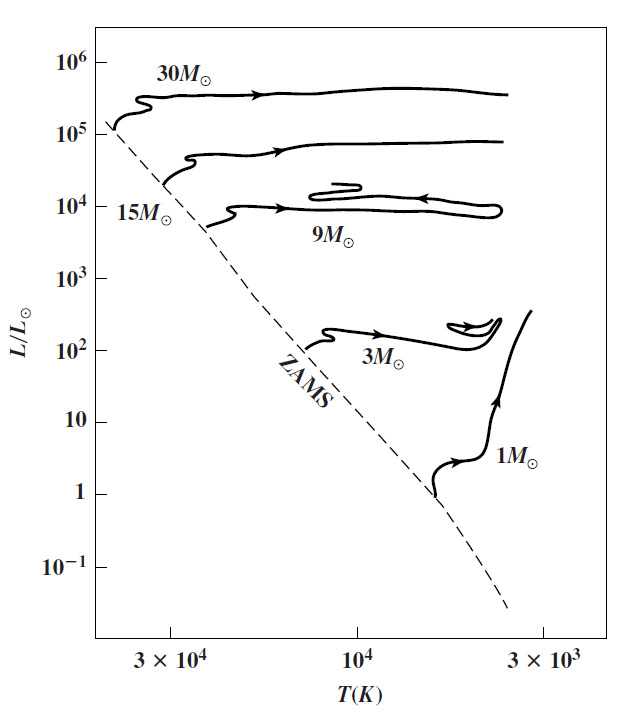
\includegraphics[scale=0.5]{Introduccion/Figures/Figura Evolucion_MS_Astronomy_Physical_Perspective.png}
	\caption{Evolución de estrellas de la secuencia principal basado en su masa
	inicial en el diagrama HR. La línea punteada representa la posición de la
	estrella en el primer momento que se integra a la secuencia principal. Al
	consumir el hidrógeno en su núcleo por las reacciones nucleares que ocurren
	en esta misma región se comienza a desatar el equilibrio delicado que
	mantiene la forma de la estrella. Esta deformación provoca una oscilación en
	su tamaño, causado por las fluctuaciones del balance entre la presión
	radiativa generada por las reacciones nucleares en el núcleo contra la
	presión gravitacional.}
	\citet{astronomyPhysicalPerspective_stellarOldAgeChapter}
	\label{evolucionMSEstrella}
\end{figure}

Aquellas estrellas cuyas masas iniciales recae bajo 8.5-10.6 \(M_{\odot}\)
terminan su vida como una estrella \textit{enana blanca.}
\citet*{whiteDwarfsReview} El ciclo de reacciones nucleares dentro del núcleo de
una estrella solo ocurre en la presencia de cierta cantidad de hidrógeno durante
su tiempo en la secuencia principal; al acabarse esta fuente de combustible la
estrella empieza a colapsar en si misma, ya que la presión radiativa del núcleo
hacia el exterior disminuye a tal grado que la presión hacia el interior de su
propia gravedad causa el encogimiento de la estrella. Esta disminución de su
radio causa que el núcleo se caliente hasta llegar a temperaturas \(T \approx
10^{8} K\) [\citet*{astronomyPhysicalPerspective_stellarOldAgeChapter}],
empezando de nuevo reacciones nucleares, esta vez involucrando el helio en vez
del hidrógeno. Estas reacciones se conocen como el proceso \textit{triple alfa},
donde tres partículas alfa \(^{4}He\) fusionan para crear un átomo de \(^{12}C\)
y un fotón gama. Mientras que en el núcleo ocurren reacciones con elementos cada
vez más pesados, el resto de los elementos más livianos (ya sea hidrógeno en el
caso de estrellas sometidas al proceso alfa u objetos más pesados como neon u
oxígeno en el caso de núcleos más densos
\citet*{astronomyPhysicalPerspective_stellarOldAgeChapter}) siguen presentes en
las capas que rodean al núcleo. La energía generada por las reacciones nucleares
dentro del núcleo se transporta a estas capas externas por medio de la radiación
generada, la cual calienta los elementos livianos, desatando de nuevo la fusión
de elementos como hidrógeno. Estas explosiones en las capas exteriores de la
estrella causa la expansión de la estrella, llegando a la fase gigante dentro
del diagrama HR.

Dependiendo de su masa inicial, una estrella puede seguir produciendo elementos
cada vez más pesados dentro de su núcleo. Sin embargo, este combustible solo le
permite a la estrella llegar hasta cierta temperatura, a partir de cual no podrá
seguir manteniendo su tasa de fusión nuclear. Una vez que llegue a este punto
empieza a expulsar las capas exteriores hasta solo dejar el núcleo expuesto,
ahora inerte debido a la ausencia de fusión nuclear. Este resto de la estrella
progenitora es lo que se conoce como la \textit{enana blanca}, a pesar de no ser
una estrella formalmente. La composición del material dentro de este objeto es
distinto al de una estrella de secuencia principal; a pesar de tener como mínimo
una masa \textapproxtilde 0.30-0.45 \(M_{\odot}\) su radio en promedio cae
dentro del mismo orden de magnitud que el radio de la Tierra.
\citet*{whiteDwarfsReview} Esto implica una densidad inmensa, en donde solo un
\textit{gas degenerado de Fermi} puede existir en estas condiciones. Un gas
degenerado surge como consecuencia del \textbf{principio de exclusión de Pauli}:
dentro de una molécula no pueden existir más de un electrón por cada estado
cuántico. Es debido a éste fenómeno que las moléculas de una estrella enana
blanca están acumuladas en un volumen varias ordenes menor comparado con una
estrella de secuencia principal, en la cual los electrones degenerados les
permiten a las moléculas almacenar más energía térmica de lo que predicen los
modelos en un gas no degenerado. Por lo tanto la escala termodinámica de una
estrella enana blanca puede llegar a ordenes de \textapproxtilde \(10^{10}\)
años, en la cual su temperatura efectiva podría disminuir de \(100,000 K\) a
\textapproxtilde \(5,000 K\). \citet*{whiteDwarfsReview}